\chapter{مطيافية الأشعة تحت الحمراء}\label{ch:g11:infrared}

على رفّ في المختبر قارورة سائل عديم اللون نُزعت عنها لصاقتها. قد يكون كحولًا،
أو \omterm{def:g11:functional-groups:carbonyl}{كيتونًا}، أو حمضًا: ثلاث عائلات تبدو متطابقة تمامًا في القارورة. قطرة توضع
على بلورة مطياف الأشعة تحت الحمراء، ودقيقتان من الانتظار، فيظهر على الشاشة
منحنى يجيب عن السؤال. فروابط \omterm{def:g7:atoms-and-molecules:molecule}{الجزيء} تهتز، وكل نوع من الروابط يمتص من الأشعة
تحت الحمراء تردداته الخاصة: \omterm{def:g11:infrared:spectrum}{وطيف الأشعة تحت الحمراء} قائمة بالروابط الموجودة.

\begin{recall}
المجموعات الوظيفية والعائلات (\cref{ch:g11:functional-groups}). ويبيّن \omterm{def:g11:absorbance:spectrum}{طيف
الامتصاص} مقدار ما تمتصه مادة من الضوء عند كل طول موجي
(\cref{ch:g11:absorbance}). وتربط الروابط الهيدروجينية مجموعات \ce{O-H}
\omterm{def:g7:atoms-and-molecules:molecule}{بالجزيئات} المجاورة (\cref{ch:g11:polarity-and-cohesion}).
\end{recall}

\section{الروابط تهتز}

\omterm{def:g10:lewis-and-shape:covalent-bond}{الرابطة التساهمية} ليست صلبة: فالذرتان تهتزان، تقتربان وتبتعدان ملايين
الملايين من المرات في الثانية، ككرتين يصل بينهما نابض. والنابض الأشد صلابة
(\omterm{def:g10:lewis-and-shape:multiple-bond}{رابطة ثنائية} بدل رابطة أحادية) أو الكرات الأخف (\omterm{def:g7:atoms-and-molecules:atom}{ذرة} هيدروجين بدل \omterm{def:g7:atoms-and-molecules:atom}{ذرة} كربون)
تهتز أسرع. ويمكن للرابطة أن تمتص أشعة تحت حمراء يوافق ترددها تردد اهتزازها:
والأشعة تحت الحمراء، غير المرئية للعين، أطوالها الموجية من بضعة ميكرومترات
إلى بضع عشرات من الميكرومترات.

\begin{omfigure}
\begin{tikzpicture}[font=\small]
  \node[aC] (c) at (0,0) {};
  \node[aO] (o) at (2.2,0) {};
  \draw[decorate, decoration={coil, aspect=0.4, segment length=4pt,
    amplitude=4pt}, thick, black!60] (c.east) -- (o.west);
  \draw[<->, omProp, thick] (-0.9,0) -- (-0.45,0);
  \draw[<->, omProp, thick] (2.65,0) -- (3.1,0);
  \node[anchor=north] at (1.1,-0.5) {رابطة تتمدد وتنكمش};
  \node[aO] (o1) at (5.3,0) {};
  \node[aH] (h1) at (6.7,0) {};
  \draw[decorate, decoration={coil, aspect=0.4, segment length=3pt,
    amplitude=3pt}, thick, black!60] (o1.east) -- (h1.west);
  \draw[<->, omProp, thick] (7.0,0) -- (7.7,0);
  \node[anchor=north, align=center] at (6.2,-0.5) {ذرة هيدروجين خفيفة:\\ اهتزاز أسرع};
\end{tikzpicture}

{\small رابطة ممثلة بنابض بين كرتين. لاهتزازها تردد تحدده صلابة الرابطة
وكتلتا الذرتين؛ والأشعة تحت الحمراء التي لها هذا التردد تُمتص.}
\end{omfigure}

\begin{definition}[العدد الموجي]\label{def:g11:infrared:wavenumber}
\emph{العدد الموجي}\index{عدد موجي} $\sigma$ لضوء ما هو مقلوب طوله الموجي،
$\sigma = 1/\lambda$. ويُعبَّر عنه في مطيافية الأشعة تحت الحمراء بالوحدة
\si{cm^{-1}}: أي عدد الأطوال الموجية في سنتيمتر واحد. فالعدد الموجي الأكبر يعني
طولًا موجيًا أقصر واهتزازًا أسرع.
\end{definition}

\begin{example}[من العدد الموجي إلى الطول الموجي]\label{ex:g11:infrared:convert}
حزمة عند $\sigma = \qty{2000}{cm^{-1}}$ توافق
$\lambda = 1/2000 = \qty{5.0e-4}{cm} = \qty{5.0}{\micro m}$. وتمتد أطياف
الأشعة تحت الحمراء عادة من \qty{4000}{cm^{-1}} (\qty{2.5}{\micro m}) إلى
\qty{500}{cm^{-1}} (\qty{20}{\micro m}).
\end{example}

\section{قراءة طيف الأشعة تحت الحمراء}

\begin{definition}[طيف الأشعة تحت الحمراء، النفاذية]\label{def:g11:infrared:spectrum}
\emph{نفاذية}\index{نفاذية} عيّنة $T$ عند \omterm{def:g11:infrared:wavenumber}{عدد موجي} معيّن هي النسبة المئوية
من الأشعة تحت الحمراء التي تجتازها: \qty{100}{\percent} إذا لم يُمتص شيء.
و\emph{طيف الأشعة تحت الحمراء}\index{طيف الأشعة تحت الحمراء} لمركب هو منحنى
$T$ بدلالة \omterm{def:g11:infrared:wavenumber}{العدد الموجي}، ويُرسم اصطلاحًا والأعداد الموجية متناقصة من اليسار
إلى اليمين.
\end{definition}

\begin{definition}[حزمة الامتصاص، منطقة البصمة]\label{def:g11:infrared:band}
\emph{حزمة الامتصاص}\index{حزمة امتصاص} انخفاض في \omterm{def:g11:infrared:spectrum}{النفاذية}: فضوء هذه الأعداد
الموجية تمتصه رابطة. وموضعها يدل على الرابطة، وعرضها وعمقها يتممان الصورة.
وتحت نحو \qty{1500}{cm^{-1}} يزدحم الطيف بحزم تتوقف على \omterm{def:g7:atoms-and-molecules:molecule}{الجزيء} كله: و\emph{منطقة
البصمة}\index{منطقة البصمة} هذه تتيح التعرف على المركب بمقارنته بطيف معروف،
لكن يصعب قراءتها رابطةً رابطةً.
\end{definition}

\begin{inthelab}[تسجيل طيف]
تستعمل معظم المطيافات في المدارس والجامعات اليوم بلورة صغيرة من الألماس: توضع
على البلورة قطرة من السائل، أو بضع حبيبات من الصلب يضغطها ملقط، وتسبر العيّنةَ
حزمةُ الأشعة تحت الحمراء التي تلامس سطح البلورة. ويُسجَّل أولًا طيف البلورة
نظيفة («الخلفية»)، وهو يؤدي دور الشاهد. وتُنظَّف البلورة بمنديل وقليل من \omterm{def:g6:solutions-and-solubility:solute}{المذيب}
بين عيّنتين.
\end{inthelab}

\section{الحزم المميِّزة}

\begin{proposition}[لكل نوع من الروابط حزمته]\label{prop:g11:infrared:bands}
% ledger: ir:OH-free, ir:OH-bonded, ir:OH-acid, ir:NH, ir:CH, ir:CO-aldehyde, ir:CO-ketone, ir:CO-ester, ir:CO-acid, ir:CC-double, ir:CO-single
يمتص كل نوع من الروابط في مجال مميِّز من الأعداد الموجية، يكاد يكون هو نفسه من
\omterm{def:g7:atoms-and-molecules:molecule}{جزيء} إلى آخر:
\begin{center}
\small
\begin{tabular}{lll}
\hline
الرابطة & \omterm{def:g11:infrared:wavenumber}{العدد الموجي} (\si{cm^{-1}}) & المظهر \\
\hline
\ce{O-H}، دون روابط هيدروجينية (غاز، \omterm{def:g2:mixing-and-dissolving:dissolve}{محلول} مخفف) & نحو 3600 & حادة \\
\ce{O-H}، بروابط هيدروجينية (\omterm{def:g11:functional-groups:alcohol}{كحول} سائل) & 3300--3400 & عريضة، قوية \\
\ce{O-H} \omterm{def:g11:functional-groups:carboxylic-acid}{لحمض كربوكسيلي} & 2500--3300 & عريضة جدًا \\
\ce{N-H} \omterm{def:g11:functional-groups:amine}{لأمين} & 3300--3500 & متوسطة (حزمتان للمجموعة \ce{-NH2}) \\
\ce{C-H} لسلسلة & 2850--2960 & قوية \\
\ce{C=O} \omterm{def:g11:functional-groups:carboxylic-acid}{لإستر} & نحو 1735 & قوية جدًا، حادة \\
\ce{C=O} \omterm{def:g11:functional-groups:carbonyl}{لألدهيد} & نحو 1730 & قوية جدًا، حادة \\
\ce{C=O} \omterm{def:g11:functional-groups:carbonyl}{لكيتون} & نحو 1715 & قوية جدًا، حادة \\
\ce{C=O} \omterm{def:g11:functional-groups:carboxylic-acid}{لحمض كربوكسيلي} & نحو 1710 & قوية جدًا، أعرض \\
\ce{C=C} & نحو 1650 & متوسطة \\
\ce{C-O} \omterm{def:g11:functional-groups:alcohol}{لكحول} & نحو 1050 & قوية \\
\hline
\end{tabular}
\end{center}
\end{proposition}

\begin{proof}
هذه المجالات مقيسة على مركبات كثيرة. وهي تتجمع بحسب الرابطة لأن اهتزاز
الرابطة يتوقف أساسًا على الرابطة نفسها وذرتيها، وقليلًا على بقية \omterm{def:g7:atoms-and-molecules:molecule}{الجزيء}.
\end{proof}

\begin{omfigure}
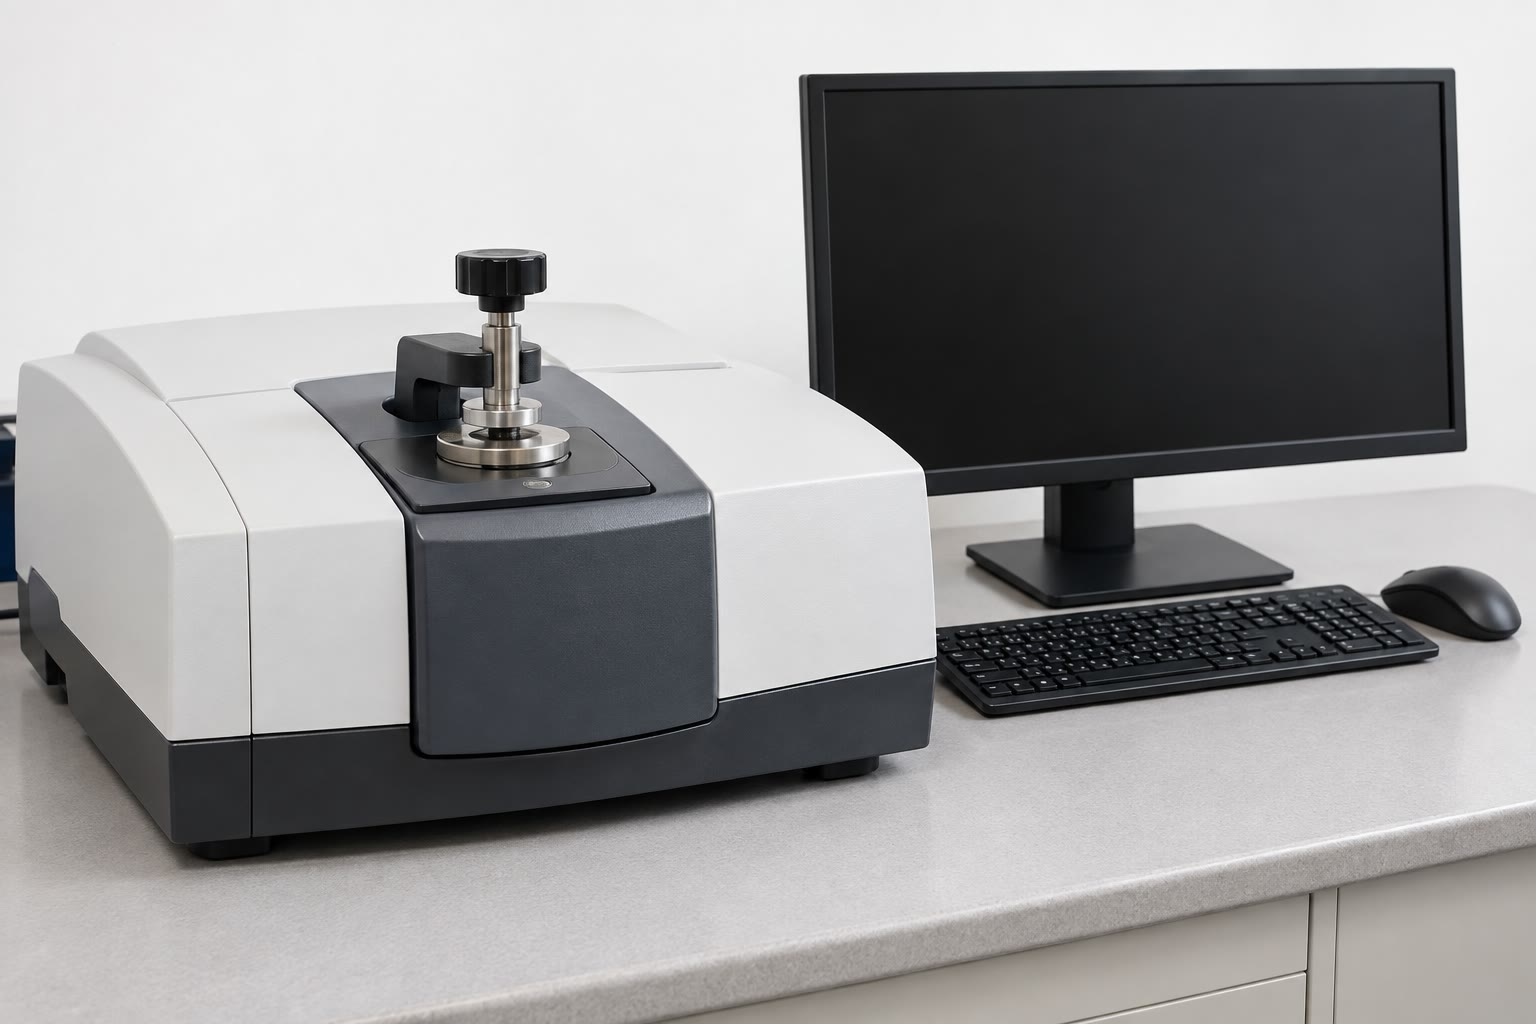
\includegraphics[width=0.48\linewidth]{images/book1/ai/g11-ftir.jpg}

{\small مطياف أشعة تحت حمراء مكتبي ببلورته وملقطه.}
\end{omfigure}

\begin{omfigure}
\begin{tikzpicture}[font=\small, x=0.0036cm, y=0.5cm]
  % wavenumber axis reversed: x = 4000 - sigma
  \fill[black!8] (2500,0.2) rectangle (3500,7.6);
  \node[font=\footnotesize, align=center, black!60] at (3000,6.8) {منطقة\\ البصمة};
  \draw[->] (0,0) -- (3600,0) node[right] {$\sigma$};
  \foreach \s in {4000,3500,3000,2500,2000,1500,1000,500}
    \draw ({4000-\s},0) -- ({4000-\s},-0.15) node[below, font=\footnotesize] {\s};
  \node[below=12pt] at (1800,-0.3) {\foreignlanguage{arabic}{العدد الموجي \babelsublr{(\si{cm^{-1}})}}};
  \foreach \a/\b/\y/\c/\l in {
      3600/3600/7/omDef/{\foreignlanguage{arabic}{\ce{O-H} حرة}},
      3300/3400/6/omDef/{\foreignlanguage{arabic}{\ce{O-H} مرتبطة}},
      2500/3300/5/omThm/{\foreignlanguage{arabic}{\ce{O-H} حمض}},
      3300/3500/4/omMeth/{\ce{N-H}},
      2850/2960/3/black!60/{\ce{C-H}},
      1700/1740/2/omProp/{\ce{C=O}},
      1050/1050/1/black!45/{\ce{C-O}}} {
    \fill[\c, rounded corners=1pt] ({4000-\b-12},{\y-0.25}) rectangle ({4000-\a+12},{\y+0.25});
    \node[anchor=west, font=\footnotesize] at ({4000-\a+40},\y) {\l};
  }
\end{tikzpicture}

{\small حيث تمتص الروابط الرئيسية. حزمتا \ce{O-H} و\ce{N-H} في اليسار،
وحزمة \ce{C=O}، وهي عادةً الأقوى، نحو \qty{1700}{cm^{-1}}؛ وتحت
\qty{1500}{cm^{-1}} تقع \omterm{def:g11:infrared:band}{منطقة البصمة}.}
\end{omfigure}

\begin{proposition}[الروابط الهيدروجينية توسّع حزمة O--H]\label{prop:g11:infrared:hbond}
% ledger: ir:OH-free, ir:OH-bonded, ir:ethanol-OH
حين ترتبط مجموعات \ce{O-H} بروابط هيدروجينية، كما في \omterm{def:g11:functional-groups:alcohol}{كحول} سائل، تكون حزمتها
عريضة وتقع عند أعداد موجية أدنى (نحو 3300--\qty{3400}{cm^{-1}})؛ ودون روابط
هيدروجينية، كما في الغاز، تكون حادة وقريبة من \qty{3600}{cm^{-1}}.
\end{proposition}

\begin{proof}
نقبله: \omterm{def:g11:polarity-and-cohesion:hydrogen-bond}{فالرابطة الهيدروجينية} تشد \omterm{def:g7:atoms-and-molecules:atom}{ذرة} الهيدروجين وتُرخي الرابطة \ce{O-H}، فتهتز
أبطأ؛ ولأن كل \omterm{def:g7:atoms-and-molecules:molecule}{جزيء} مرتبط على نحو يختلف قليلًا، تنتشر الحزمة على مجال.
\end{proof}

\section{التعرف على المجموعات الوظيفية}


\begin{method}[قراءة طيف الأشعة تحت الحمراء]\label{met:g11:infrared:reading}
\begin{enumerate}
  \item انظر أولًا فوق \qty{1500}{cm^{-1}}؛ واترك \omterm{def:g11:infrared:band}{منطقة البصمة}
        للمقارنة بأطياف معروفة.
  \item نحو \qty{1700}{cm^{-1}}: حزمة قوية جدًا تعني مجموعة \ce{C=O}
        (\omterm{def:g11:functional-groups:carbonyl}{ألدهيد}، \omterm{def:g11:functional-groups:carbonyl}{كيتون}، حمض، \omterm{def:g11:functional-groups:carboxylic-acid}{إستر}، \omterm{def:g11:functional-groups:amine}{أميد}).
  \item بين 2500 و\qty{3700}{cm^{-1}}: حزمة عريضة نحو
        \qty{3350}{cm^{-1}} تعني \ce{O-H} \omterm{def:g11:functional-groups:alcohol}{كحول}؛ وحزمة عريضة جدًا
        من 2500 إلى \qty{3300}{cm^{-1}} مع \ce{C=O} تعني
        حمضًا كربوكسيليًا؛ وحزم متوسطة عند 3300--\qty{3500}{cm^{-1}} تعني
        \ce{N-H}.
  \item اجمع ذلك إلى \omterm{def:g11:organic-skeletons:formulas}{الصيغة الجزيئية} لتختار العائلة، ثم
        تحقق بموضع حزمة \ce{C=O} إن وُجدت.
\end{enumerate}
\end{method}

\begin{omfigure}
\newcommand{\irpanel}[2]{%
\begin{tikzpicture}
\begin{axis}[width=0.96\linewidth, height=3.9cm, x dir=reverse, xmin=500,
    xmax=4000, ymin=0, ymax=105, xtick={4000,3000,2000,1000},
    /pgf/number format/1000 sep={},
    ytick={0,50,100}, tick label style={font=\scriptsize},
    label style={font=\scriptsize}, ylabel={\babelsublr{$T$ (\%)}}, axis lines*=left,
    title={\small #2}, title style={yshift=-4pt}]
  \addplot[thick, omDef] table[x=sigma, y=#1] {figdata/out/grade-11-infrared.dat};
\end{axis}
\end{tikzpicture}}
\begin{minipage}{0.49\linewidth}\irpanel{ethanolL}{A: الإيثانول (سائل)}\end{minipage}\hfill
\begin{minipage}{0.49\linewidth}\irpanel{ethanolG}{B: الإيثانول (غاز)}\end{minipage}

\begin{minipage}{0.49\linewidth}\irpanel{propanone}{C: البروبانون}\end{minipage}\hfill
\begin{minipage}{0.49\linewidth}\irpanel{acid}{D: حمض الإيثانويك}\end{minipage}

\begin{minipage}{0.49\linewidth}\irpanel{ester}{E: إيثانوات الإيثيل}\end{minipage}\hfill
\begin{minipage}{0.49\linewidth}\irpanel{amine}{F: الإيثان \omterm{def:g11:functional-groups:amine}{أمين}}\end{minipage}

{\small أطياف الأشعة تحت الحمراء لستة مركبات، \omterm{def:g11:infrared:wavenumber}{والعدد الموجي} بالوحدة \si{cm^{-1}}
(متناقص نحو اليمين). لم تُرسم إلا الحزم المذكورة في الفصل؛ ومواضعها مأخوذة من
أطياف مقيسة ومن جداول، وأشكالها من نموذج بسيط.}
\end{omfigure}

\begin{example}[قراءة الأطياف الستة]\label{ex:g11:infrared:six}
% ledger: ir:OH-bonded, ir:ethanol-OH, ir:CO-ketone, ir:OH-acid, ir:CO-acid, ir:CO-ester, ir:ethylethanoate-COC, ir:NH
يُظهر الإيثانول (A) حزمة \ce{O-H} عريضة نحو \qty{3350}{cm^{-1}}، وحزم
\ce{C-H} تحت \qty{3000}{cm^{-1}} بقليل، وحزمة \ce{C-O} قوية
نحو \qty{1050}{cm^{-1}}، لكن لا شيء نحو \qty{1700}{cm^{-1}}. وفي
الغاز (B) تصير حزمة \ce{O-H} خطًا حادًا عند
\qty{3666}{cm^{-1}}. وليس للبروبانون (C) حزمة \ce{O-H} لكن له حزمة
\ce{C=O} قوية جدًا عند \qty{1715}{cm^{-1}}. ويُظهر حمض الإيثانويك (D) الاثنتين:
حزمة \ce{O-H} هائلة من 2500 إلى \qty{3300}{cm^{-1}} وحزمة \ce{C=O}
عند \qty{1710}{cm^{-1}}. ولإيثانوات الإيثيل (E) حزمة \ce{C=O} عند
\qty{1735}{cm^{-1}} وحزمة \ce{C-O} قوية نحو \qty{1240}{cm^{-1}}، ولا
حزمة \ce{O-H}. ويُظهر الإيثان \omterm{def:g11:functional-groups:amine}{أمين} (F) حزمتي \ce{N-H} متوسطتين فوق
\qty{3300}{cm^{-1}}.
\end{example}

\section{تمارين}

\begin{exercise}[$\star$]\label{exo:g11:infrared:1}
حوّل إلى طول موجي بالميكرومتر: $\sigma = \qty{3300}{cm^{-1}}$
و$\sigma = \qty{1050}{cm^{-1}}$. أيهما يوافق الاهتزاز
الأسرع؟
\end{exercise}

\begin{exercise}[$\star$]\label{exo:g11:infrared:2}
يُمتص طول موجي قدره \qty{10}{\micro m}. أعطِ \omterm{def:g11:infrared:wavenumber}{العدد الموجي}
بالوحدة \si{cm^{-1}}.
\end{exercise}

\begin{exercise}[$\star$]\label{exo:g11:infrared:3}
أي رابطة تمتص: نحو \qty{1715}{cm^{-1}}؛ ونحو \qty{3350}{cm^{-1}}
(حزمة عريضة)؛ وبين 2850 و\qty{2960}{cm^{-1}}؟
\end{exercise}

\begin{exercise}[$\star$]\label{exo:g11:infrared:4}
جد في الطيف C (البروبانون) أقوى حزمة. إلى أي رابطة
تعود؟
\end{exercise}

\begin{exercise}[$\star$]\label{exo:g11:infrared:5}
لماذا يُرسم \omterm{def:g11:infrared:spectrum}{طيف الأشعة تحت الحمراء} بمحور \omterm{def:g11:infrared:spectrum}{نفاذية}، والحزم متجهة
إلى الأسفل؟ وماذا يعني $T = \qty{100}{\percent}$؟
\end{exercise}

\begin{exercise}[$\star\star$]\label{exo:g11:infrared:6}
يُظهر مركب \ce{C4H8O} حزمة قوية جدًا عند
\qty{1715}{cm^{-1}} ولا حزمة فوق \qty{3000}{cm^{-1}}. ويُظهر مركب آخر،
\ce{C4H10O}، حزمة عريضة نحو \qty{3350}{cm^{-1}} ولا شيء نحو
\qty{1700}{cm^{-1}}. إلى أي عائلتين ينتميان؟ واقترح اسمًا
لكل منهما.
\end{exercise}

\begin{exercise}[$\star\star$]\label{exo:g11:infrared:7}
اشرح لماذا حزمة \ce{O-H} لحمض الإيثانويك عريضة إلى هذا الحد، بل أعرض
من حزمة الإيثانول السائل.
\end{exercise}

\begin{exercise}[$\star\star$]\label{exo:g11:infrared:8}
قارن الطيفين A وB للإيثانول. ماذا يتغير، ولماذا؟
\end{exercise}

\begin{exercise}[$\star\star$]\label{exo:g11:infrared:9}
البروبانال والبروبانون كلاهما \ce{C3H6O}. ولكليهما حزمة \ce{C=O}
قوية. أيمكن للأشعة تحت الحمراء أن تميّز بينهما بهذه الحزمة وحدها؟ وما الذي
قد يساعد أيضًا؟
\end{exercise}

\begin{exercise}[$\star\star$]\label{exo:g11:infrared:10}
يُظهر مركب حزمة قوية عند \qty{1735}{cm^{-1}}، وحزمة قوية نحو
\qty{1240}{cm^{-1}}، ولا شيء فوق \qty{3000}{cm^{-1}}. وصيغته
\ce{C4H8O2}. ما عائلته؟ أيمكن أن يكون حمض الإيثانويك؟ أو حمض
البوتانويك؟
\end{exercise}

\begin{exercise}[$\star\star$]\label{exo:g11:infrared:11}
أي الأطياف الستة يشبه أكثر طيفُ \omterm{def:g7:atoms-and-molecules:molecule}{جزيء} بروبان-1-ول؟ وطيفُ حمض
البروبانويك؟ اشرح.
\end{exercise}

\begin{exercise}[$\star\star\star$]\label{exo:g11:infrared:12}
يمكن أكسدة بروبان-2-ول إلى بروبانون. وتتابع طالبة
التفاعل بتسجيل أطياف عيّنات تؤخذ كل عشر دقائق.
صف كيف تتغير الأطياف. وكيف تعرف أن التفاعل
قد اكتمل؟
\end{exercise}

\begin{exercise}[$\star\star\star$]\label{exo:g11:infrared:13}
حمض البوتانويك وإيثانوات الإيثيل متماكبان، \ce{C4H8O2}. صف فرقين
بين طيفيهما في الأشعة تحت الحمراء، واشرحهما.
\end{exercise}

\begin{exercise}[$\star\star\star$]\label{exo:g11:infrared:14}
تُظهر عيّنة من إيثانوات الإيثيل، إلى جانب الحزم المتوقعة، حزمة ضعيفة
عريضة نحو \qty{3350}{cm^{-1}}. اقترح شائبتين يمكن أن
تسببها (فكّر في طريقة صنع \omterm{def:g11:functional-groups:carboxylic-acid}{الإسترات}، وفي \omterm{def:g4:air-a-mixture-of-gases:air}{الهواء}). وكيف يمكن التحقق من
العيّنة؟
\end{exercise}

\begin{exercise}[$\star\star\star$]\label{exo:g11:infrared:15}
تقع حزمة \ce{C=O} للكيتونات نحو \qty{1715}{cm^{-1}}، وحزمة
\ce{C=C} نحو \qty{1650}{cm^{-1}}، وحزمة \ce{C-O} نحو
\qty{1050}{cm^{-1}}. مستعينًا بصورة الكرتين على نابض، اشرح
لماذا تهتز \omterm{def:g10:lewis-and-shape:multiple-bond}{الرابطة الثنائية} \ce{C=O} أسرع من الرابطة الأحادية \ce{C-O}.
ولماذا تقع حزم \ce{O-H} و\ce{N-H} و\ce{C-H} كلها عند أعداد موجية عالية؟
\end{exercise}

\section{مسألة: ثلاث قوارير بلا لصاقات}

\begin{problem}[{مسألة نهاية الأسبوع --- ثلاث قوارير فقدت لصاقاتها:
أيها أيها، وما الطول الموجي الذي يمتصه الكيتون أكثر من غيره؟}]
\label{pb:g11:infrared:1}
% ledger: ir:OH-bonded, ir:OH-acid, ir:CO-ketone, ir:CO-acid, ir:CO-single
فقدت ثلاث قوارير من سائل عديم اللون لصاقاتها. وتقول قائمة المخزون
إنها تحوي الإيثانول والبروبانون وحمض الإيثانويك. تُسجَّل أطيافها:
فتعطي القارورة 1 طيفًا يشبه A، والقارورة 2 طيفًا يشبه D، والقارورة 3
طيفًا يشبه C.

\medskip
\noindent\textbf{الجزء الأول --- المرشحات.}
\begin{enumerate}
  \item اكتب الصيغ نصف البنيوية للإيثانول والبروبانون
        وحمض الإيثانويك.
  \item أعطِ صيغها الجزيئية.
  \item سمِّ \omterm{def:g11:functional-groups:functional-group}{المجموعة الوظيفية} لكل منها.
  \item أي روابط كل منها ينبغي أن تعطي حزمة فوق
        \qty{1500}{cm^{-1}}؟
\end{enumerate}

\medskip
\noindent\textbf{الجزء الثاني --- الأطياف.}
\begin{enumerate}[resume]
  \item القارورة 1: أفيها حزمة \ce{C=O}؟ وحزمة \ce{O-H}؟ وأي
        مركب هي؟
  \item القارورة 2: صف أبرز سمتين فيها. وأي مركب هي؟
  \item القارورة 3: أي مركب هي؟ وأي حزمة تحسم ذلك؟
  \item أكانت الرائحة تكفي للتمييز بينها؟ ولماذا الأفضل ألا
        يُجرَّب ذلك؟
  \item لماذا حزمة \ce{O-H} للقارورة 2 أعرض من حزمة القارورة 1؟
\end{enumerate}

\medskip
\noindent\textbf{الجزء الثالث --- \omterm{def:g11:organic-skeletons:isomer}{المتماكبات}.}
\begin{enumerate}[resume]
  \item الميثوكسي ميثان متماكب للإيثانول. اكتب صيغته. وأي
        حزمة من حزم الإيثانول تغيب عن طيفه؟
  \item البروبانال متماكب للبروبانون. أي حزمة يشتركان فيها؟
        وأين تقع لكل منهما؟
  \item ميثانوات الميثيل، \ce{HCOO-CH3}، متماكب لحمض الإيثانويك.
        أي حزمة من حزم الحمض تغيب؟ وأين تقع حزمته
        \ce{C=O}؟
  \item لماذا لا تكفي \omterm{def:g11:organic-skeletons:formulas}{الصيغة الجزيئية} وحدها للتعرف على مركب، في حين
        تكفي الصيغة والطيف معًا في الغالب؟
\end{enumerate}

\medskip
\noindent\textbf{الجزء الرابع --- الطول الموجي.}
\begin{enumerate}[resume]
  \item ما \omterm{def:g11:infrared:wavenumber}{العدد الموجي} لأقوى حزمة في طيف البروبانون؟
  \item عبّر عنه بالوحدة \si{m^{-1}}.
  \item احسب الطول الموجي الممتص، بالمتر، ثم
        بالميكرومتر.
  \item أهذا الضوء مرئي؟ وإلى أي نوع من الإشعاع
        ينتمي؟
  \item افعل الشيء نفسه لحزمة \ce{C-O} للإيثانول نحو
        \qty{1050}{cm^{-1}}.
  \item أي الرابطتين تهتز أسرع؟
  \item اذكر الجواب النهائي: ما الطول الموجي الذي تمتصه الرابطة \ce{C=O}
        في البروبانون أكثر من غيره؟
\end{enumerate}
\end{problem}
